% --
% Speech Commands dataset

\subsection{Speech Commands Dataset}\label{sec:exp_dataset_speech_cmd}
The speech command dataset \cite{Warden2018} is a very diverse dataset consisting of over thousands of different speakers. This dataset is by any means no clean dataset recorded by professionals, if anything it is the opposite.
Some information on how the dataset is created is shown in \cite{Warden2018}, where also some quality check of the recorded files has been done to reject bad samples.
However there are still many flaws such as that the audio files are not normalized, too loud or too silent files or with inconsistent sample numbers and some examples are prone with too much noise or even noise only.
Still it is a great dataset, because there is no need for a perfect dataset when working with neural networks and one can be happy that there exists one with this amount of diversity and free of access.
In fact maybe its even better to have an unclean dataset, so that invariances against noise are learnt during training.
Some examples in raw audio format are shown in \rfig{exp_dataset_wav_grid_c30}.
\begin{figure}[!ht]
  \centering
    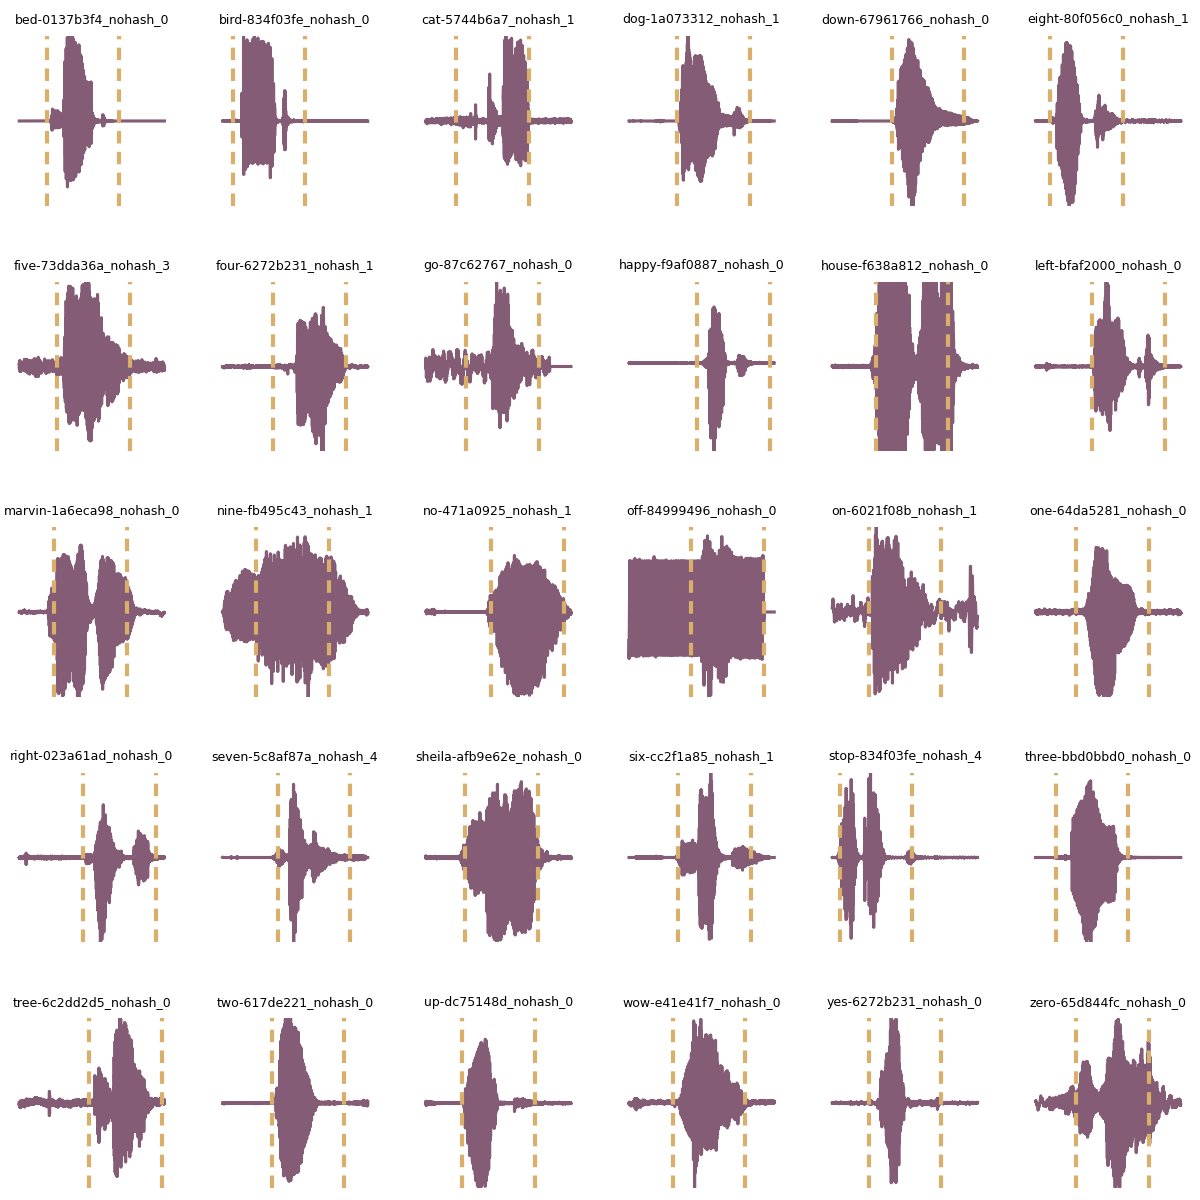
\includegraphics[width=0.65\textwidth]{./5_exp/figs/exp_dataset_wav_grid_c30}
  \caption{Random samples from the Speech Command Dataset, one per class. Pre-processed and normalized raw audio data.}
  \label{fig:exp_dataset_wav_grid_c30}
\end{figure}
\FloatBarrier
\noindent

